\documentclass[10pt]{article}
\usepackage[margin=2.1cm]{geometry}
\usepackage{graphicx,booktabs,xcolor,enumitem,amsmath,caption,float,tabularx,microtype,array}
\usepackage{hyperref}
\hypersetup{colorlinks=true, urlcolor={blue!70!black}, linkcolor=black, citecolor=black, filecolor=black}
\usepackage{tikz}
\usetikzlibrary{arrows.meta,positioning,shapes.geometric,fit,backgrounds,calc}
\usepackage{listings}
\lstset{basicstyle=\ttfamily\footnotesize,breaklines=true,columns=fullflexible,frame=single,framesep=3pt,
        rulecolor=\color{gray!50},backgroundcolor=\color{gray!5}}
\setlist{itemsep=1pt,topsep=3pt,parsep=0pt}
\captionsetup{font=small,labelfont=bf}
\graphicspath{{../figs/}}
\newcommand{\numAexbkgpe}{1,179,934}
\newcommand{\numAexbkgperus}{125}
\newcommand{\numAexmarleype}{205}
\newcommand{\numAmixhits}{12,929}
\newcommand{\numAmixmarley}{588}
\newcommand{\numAmixpe}{1,171,788}
\newcommand{\numAmixsamples}{93.7}
\newcommand{\numAmixsnip}{221,591}
\newcommand{\numAsolhits}{9}
\newcommand{\numAsolmarley}{490}
\newcommand{\numAsolpe}{508}
\newcommand{\numAsolsamples}{0.0}
\newcommand{\numAsolsnip}{81}
\newcommand{\numBdefaultmixagain}{0.07}
\newcommand{\numBdefaultmixdedhits}{211,736}
\newcommand{\numBdefaultmixdedupe}{5,295,985}
\newcommand{\numBdefaultmixduphits}{0.00}
\newcommand{\numBdefaultmixduppe}{0.00}
\newcommand{\numBdefaultmixhitpe}{5,295,985}
\newcommand{\numBdefaultmixhits}{211,736}
\newcommand{\numBdefaultmixrms}{2.50}
\newcommand{\numBdefaultmixsamples}{1373.2}
\newcommand{\numBdefaultmixsnip}{3,358,352}
\newcommand{\numBdefaultsolagain}{0.01}
\newcommand{\numBdefaultsoldedhits}{178}
\newcommand{\numBdefaultsoldedupe}{3,309}
\newcommand{\numBdefaultsolduphits}{0.00}
\newcommand{\numBdefaultsolduppe}{0.00}
\newcommand{\numBdefaultsolhitpe}{3,309}
\newcommand{\numBdefaultsolhits}{178}
\newcommand{\numBdefaultsolrms}{2.49}
\newcommand{\numBdefaultsolsamples}{0.5}
\newcommand{\numBdefaultsolsnip}{1,505}
\newcommand{\numBfixBmixagain}{0.07}
\newcommand{\numBfixBmixdedhits}{218,038}
\newcommand{\numBfixBmixdedupe}{5,348,590}
\newcommand{\numBfixBmixduphits}{0.00}
\newcommand{\numBfixBmixduppe}{0.00}
\newcommand{\numBfixBmixhitpe}{5,348,590}
\newcommand{\numBfixBmixhits}{218,038}
\newcommand{\numBfixBmixrms}{2.50}
\newcommand{\numBfixBmixsamples}{1444.8}
\newcommand{\numBfixBmixsnip}{3,477,944}
\newcommand{\numBfixBsolagain}{0.00}
\newcommand{\numBfixBsoldedhits}{178}
\newcommand{\numBfixBsoldedupe}{3,303}
\newcommand{\numBfixBsolduphits}{0.00}
\newcommand{\numBfixBsolduppe}{0.00}
\newcommand{\numBfixBsolhitpe}{3,303}
\newcommand{\numBfixBsolhits}{178}
\newcommand{\numBfixBsolrms}{2.50}
\newcommand{\numBfixBsolsamples}{0.6}
\newcommand{\numBfixBsolsnip}{1,622}
\newcommand{\numBlegacymixagain}{15.66}
\newcommand{\numBlegacymixdedhits}{226,600}
\newcommand{\numBlegacymixdedupe}{5,605,068}
\newcommand{\numBlegacymixduphits}{12.38}
\newcommand{\numBlegacymixduppe}{15.94}
\newcommand{\numBlegacymixhitpe}{6,667,749}
\newcommand{\numBlegacymixhits}{258,620}
\newcommand{\numBlegacymixrms}{2.74}
\newcommand{\numBlegacymixsamples}{1873.5}
\newcommand{\numBlegacymixsnip}{4,431,828}
\newcommand{\numBlegacysolagain}{0.10}
\newcommand{\numBlegacysoldedhits}{181}
\newcommand{\numBlegacysoldedupe}{3,320}
\newcommand{\numBlegacysolduphits}{0.00}
\newcommand{\numBlegacysolduppe}{0.00}
\newcommand{\numBlegacysolhitpe}{3,320}
\newcommand{\numBlegacysolhits}{181}
\newcommand{\numBlegacysolrms}{2.52}
\newcommand{\numBlegacysolsamples}{0.6}
\newcommand{\numBlegacysolsnip}{1,621}
\newcommand{\numBstockmixagain}{15.66}
\newcommand{\numBstockmixdedhits}{226,641}
\newcommand{\numBstockmixdedupe}{5,639,007}
\newcommand{\numBstockmixduphits}{12.38}
\newcommand{\numBstockmixduppe}{15.85}
\newcommand{\numBstockmixhitpe}{6,701,517}
\newcommand{\numBstockmixhits}{258,657}
\newcommand{\numBstockmixrms}{2.74}
\newcommand{\numBstockmixsamples}{1873.5}
\newcommand{\numBstockmixsnip}{4,431,828}
\newcommand{\numBstocksolagain}{0.10}
\newcommand{\numBstocksoldedhits}{181}
\newcommand{\numBstocksoldedupe}{3,320}
\newcommand{\numBstocksolduphits}{0.00}
\newcommand{\numBstocksolduppe}{0.00}
\newcommand{\numBstocksolhitpe}{3,320}
\newcommand{\numBstocksolhits}{181}
\newcommand{\numBstocksolrms}{2.52}
\newcommand{\numBstocksolsamples}{0.6}
\newcommand{\numBstocksolsnip}{1,621}
\newcommand{\numCallmixmarley}{13,178}
\newcommand{\numCallmixratio}{0.214}
\newcommand{\numCallmixtotal}{28,261,229}
\newcommand{\numCallsolmarley}{10,281}
\newcommand{\numCallsolratio}{0.224}
\newcommand{\numCallsoltotal}{10,627}
\newcommand{\numCdefaultmixmarley}{11,886}
\newcommand{\numCdefaultmixratio}{0.139}
\newcommand{\numCdefaultmixtotal}{23,437,995}
\newcommand{\numCdefaultsolmarley}{9,781}
\newcommand{\numCdefaultsolratio}{0.186}
\newcommand{\numCdefaultsoltotal}{10,135}
\newcommand{\numCfixCmixmarley}{13,009}
\newcommand{\numCfixCmixratio}{0.210}
\newcommand{\numCfixCmixtotal}{28,263,680}
\newcommand{\numCfixCsolmarley}{10,279}
\newcommand{\numCfixCsolratio}{0.225}
\newcommand{\numCfixCsoltotal}{10,639}
\newcommand{\numCgainmixmarley}{10.6}
\newcommand{\numCgainmixratio}{0.655}
\newcommand{\numCgainmixtotal}{20.6}
\newcommand{\numCgainsolmarley}{5.0}
\newcommand{\numCgainsolratio}{0.837}
\newcommand{\numCgainsoltotal}{4.7}
\newcommand{\numClegacymixmarley}{11,765}
\newcommand{\numClegacymixratio}{0.138}
\newcommand{\numClegacymixtotal}{23,435,770}
\newcommand{\numClegacysolmarley}{9,791}
\newcommand{\numClegacysolratio}{0.188}
\newcommand{\numClegacysoltotal}{10,162}
\newcommand{\numCstockmixmarley}{11,765}
\newcommand{\numCstockmixratio}{0.138}
\newcommand{\numCstockmixtotal}{23,435,770}
\newcommand{\numCstocksolmarley}{9,791}
\newcommand{\numCstocksolratio}{0.188}
\newcommand{\numCstocksoltotal}{10,162}
\newcommand{\numDfixDmax}{4247.85}
\newcommand{\numDfixDmin}{-4040.64}
\newcommand{\numDfixDn}{1,541}
\newcommand{\numDfixDnear}{0.2}
\newcommand{\numDlegacymax}{4.25}
\newcommand{\numDlegacymin}{-4.04}
\newcommand{\numDlegacyn}{1,541}
\newcommand{\numDlegacynear}{100.0}
\newcommand{\numDperevent}{38.5}
\newcommand{\numElegacymixfirst}{193}
\newcommand{\numElegacymixhits}{0}
\newcommand{\numElegacymixsnip}{0}
\newcommand{\numElegacysolfirst}{0}
\newcommand{\numElegacysolhits}{0}
\newcommand{\numElegacysolsnip}{0}
\newcommand{\numEstockmixfirst}{5}
\newcommand{\numEstockmixhits}{69}
\newcommand{\numEstockmixsnip}{188}
\newcommand{\numEstocksolfirst}{0}
\newcommand{\numEstocksolhits}{0}
\newcommand{\numEstocksolsnip}{0}
\newcommand{\numEwrapvalue}{$2.95\times10^{17}$}
\newcommand{\numNfixNOnePZero}{0.627}
\newcommand{\numNfixNOnePgt}{7.5}
\newcommand{\numNfixNOnecells}{38,231,097}
\newcommand{\numNfixNOnevm}{1.03}
\newcommand{\numNlegacyPZero}{0.689}
\newcommand{\numNlegacyPgt}{10.6}
\newcommand{\numNlegacycells}{38,231,097}
\newcommand{\numNlegacyvm}{1.50}
\newcommand{\numNmix}{20}
\newcommand{\numNpredbinomial}{0.627}
\newcommand{\numNpredpoisson}{0.689}
\newcommand{\numNq}{0.373}
\newcommand{\numNsol}{20}
\newcommand{\numOallmixhitpe}{6,473,104}
\newcommand{\numOallmixhits}{259,223}
\newcommand{\numOallmixmarley}{13,178}
\newcommand{\numOallmixpe}{28,261,229}
\newcommand{\numOallsolhitpe}{3,498}
\newcommand{\numOallsolhits}{175}
\newcommand{\numOallsolmarley}{10,281}
\newcommand{\numOallsolpe}{10,627}
\newcommand{\numOdefaultmixhitpe}{5,295,985}
\newcommand{\numOdefaultmixhits}{211,736}
\newcommand{\numOdefaultmixmarley}{11,886}
\newcommand{\numOdefaultmixpe}{23,437,995}
\newcommand{\numOdefaultsolhitpe}{3,309}
\newcommand{\numOdefaultsolhits}{178}
\newcommand{\numOdefaultsolmarley}{9,781}
\newcommand{\numOdefaultsolpe}{10,135}
\newcommand{\numOstockmixhitpe}{6,667,039}
\newcommand{\numOstockmixhits}{258,588}
\newcommand{\numOstockmixmarley}{11,765}
\newcommand{\numOstockmixpe}{23,435,770}
\newcommand{\numOstocksolhitpe}{3,320}
\newcommand{\numOstocksolhits}{181}
\newcommand{\numOstocksolmarley}{9,791}
\newcommand{\numOstocksolpe}{10,162}
\newcommand{\numgateBdiv}{40/40}
\newcommand{\numgateBidentmix}{0/20}
\newcommand{\numgateBidentsol}{17/20}
\newcommand{\numgateBidentnolapmix}{yes}
\newcommand{\numgateBidentnolapsol}{yes}
\newcommand{\numgateBnolapmix}{0/20}
\newcommand{\numgateBnolapsol}{13/20}
\newcommand{\numgateCxe}{40/40}
\newcommand{\numgateEonly}{40/40}
\newcommand{\numgatelegacydiveq}{40/40}
\newcommand{\numgatestockeqstored}{40/40}


\newcommand{\code}[1]{\texttt{#1}}
\newcommand{\fn}[1]{\nolinkurl{#1}}
\makeatletter\g@addto@macro{\UrlBreaks}{\do\_\do/\do-\do.}\makeatother
\newcommand{\us}{\,\textmu s}
\newcommand{\ns}{\,ns}
\definecolor{bef}{HTML}{c0392b}
\definecolor{aft}{HTML}{2471a3}
\newcommand{\bugbox}[3]{%
\noindent\fcolorbox{gray!60}{gray!6}{\parbox{\dimexpr\linewidth-2\fboxsep-2\fboxrule}{\small
\textbf{What goes wrong.} #1\par\smallskip
\textbf{Impact.} #2\par\smallskip
\textbf{Fix.} #3}}\par\medskip}

\title{\textbf{The DUNE FD-VD light simulation for low-energy physics:\\
workflow, five simulation bugs, and proposed fixes}}
\author{Haiwang Yu\\[2pt]
\small Bugs B, C, D, E and N1 were found by Xin Qian (fdvd\_sim studies, \href{https://github.com/WireCell/wcp-porting-validation/tree/main/fdvd_sim/docs}{\code{WireCell/wcp-porting-validation}});\\
\small this note reproduces them, fixes them in \code{duneopdet}, and measures the effect of each fix.}
\date{Draft, \today}

\begin{document}
\maketitle

\begin{abstract}
\noindent
The photon-detector (light) simulation of the DUNE far detector has five bugs in two \code{duneopdet} modules,
\code{SIPMOpSensorSim} and \code{WaveformDigitizerSim}. Two of them only matter when several interactions share one
readout, which is exactly the situation of low-energy (solar, supernova) physics, where a neutrino sits on top of the
radiological background. In FD-VD solar events simulated with the official configuration and background,
\numBlegacymixduphits\,\% of the OpHits are copies of other OpHits, and the neutrino's argon light is
\numCgainmixratio\ of what a per-track late-light reference gives; neither effect exists in signal-only samples, so a calibration made on
signal-only samples is biased for real conditions. This note (1) explains in plain language what the low-energy
light workflow is and how it differs from the beam workflow, (2) gives a minimum gen\,$\to$\,Geant4\,$\to$\,detsim
workflow that reproduces every bug in about an hour, and (3) for each bug shows the effect before and after a proposed
fix on \numNsol\ signal-only and \numNmix\ signal-plus-background events. The fixes are one patch to \code{duneopdet}
(it applies to \code{v10\_26\_00d00} and to \code{develop}); every fix can be switched off to reproduce existing
samples bit for bit.
\end{abstract}

\tableofcontents
\bigskip

%=====================================================================================================================
\section{Summary for the conveners}
%=====================================================================================================================

Table~\ref{tab:summary} lists the bugs. The letters follow Xin Qian's numbering (fdvd\_sim doc~30), so they can be
cross-referenced with his notes. ``Mixed'' means a MARLEY solar-$\nu_e$ event plus the nominal DUNE radiological model
in the same readout; ``solar-only'' means the MARLEY event alone.

\begin{table}[H]\centering\small
\caption{The five bugs, their size in our samples before (\textcolor{bef}{legacy}) and after
(\textcolor{aft}{fixed}) the fix, and the proposed default. Numbers are totals over the \numNmix\ mixed and \numNsol\
solar-only events of section~\ref{sec:bugs}.}
\label{tab:summary}
\renewcommand{\arraystretch}{1.15}
\begin{tabularx}{\linewidth}{@{}l >{\raggedright\arraybackslash\footnotesize}p{3.05cm} >{\raggedright\arraybackslash}X >{\raggedright\arraybackslash}p{4.1cm} >{\raggedright\arraybackslash}p{1.3cm}@{}}
\toprule
 & module & what goes wrong & size, before $\to$ after & default \\
\midrule
B & \code{WaveformDigitizerSim} & overlapping ``focus ranges'': the same waveform samples are stored twice and
  get the noise twice & dup.\ OpHits \numBlegacymixduphits\,\% $\to$ \numBfixBmixduphits\,\% (mixed) & fix on \\
C & \code{SIPMOpSensorSim} & ``late light'' is timed from the first photon of the whole event, not of the
  interaction & MARLEY Ar PE/photon \numClegacymixratio\ $\to$ \numCfixCmixratio\ (mixed) & opt-in \\
D & \code{SIPMOpSensorSim} & dark-count times are in \textmu s but stored as ns & \numDlegacynear\,\% $\to$
  \numDfixDnear\,\% of dark counts within $\pm5$\us\ of the $\nu$ & fix on \\
E & \code{WaveformDigitizerSim} & unsigned underflow of the readout start at the beginning of the window
  & \numEstockmixsnip\ $\to$ \numElegacymixsnip\ snippets at \numEwrapvalue\us & always \\
N1 & \code{SIPMOpSensorSim} & photon detection is a second Poisson draw instead of a binomial one &
  P(0\,PE\,$|$\,1 photon) \numNlegacyPZero\ $\to$ \numNfixNOnePZero & fix on \\
\bottomrule
\end{tabularx}
\end{table}

\begin{itemize}
\item \textbf{B and C are pile-up bugs.} They need several interactions in one readout and are absent in signal-only
  samples. They change the light of the \emph{signal} in mixed events, not only the background.
\item \textbf{D, E and N1 act in every event.} D moves the dark counts onto the neutrino flash. E creates a handful of
  waveform snippets with a nonsense time stamp (and reads memory outside the waveform buffer). N1 makes the photon
  counting statistics too wide.
\item \textbf{Proposal.} One commit on branch \code{fix-light-sim-pileup} of
  \href{https://github.com/HaiwangYu/duneopdet/tree/fix-light-sim-pileup}{\code{github.com/HaiwangYu/duneopdet}},
  on top of \code{DUNE/duneopdet} \code{develop} (appendix~\ref{app:patch}). B, D and N1 are fixed by default with a switch back to
  the legacy behaviour; E has no switch (the legacy output is undefined behaviour); C changes the light model and is
  opt-in (\code{LateLightReference: "Track"}), to be decided by the photon-detector simulation experts.
\item \textbf{Other known issues} of the same chain, not fixed here, are listed in section~\ref{sec:other}. The
  largest light loss in the chain is not a bug but a setting of the OpHit finder (F in that list).
\end{itemize}

%=====================================================================================================================
\section{Low-energy versus beam physics, in plain words}
\label{sec:le}
%=====================================================================================================================

\paragraph{Beam neutrinos.} The accelerator sends a short spill of neutrinos every $\sim$1\,s, and we know exactly when.
The detector is read out around the spill time. A beam neutrino interaction deposits GeV of energy, produces long
tracks and showers, and gives a big flash of scintillation light. Radioactive decays in the argon also happen during
the readout, but they deposit only MeV each, far below the beam event, so they barely matter. In simulation, one
event is usually one neutrino interaction at $t=0$.

\paragraph{Low-energy neutrinos (solar, supernova).} A solar $\nu_e$ interacting by charged current on argon
($\nu_e + {}^{40}\mathrm{Ar} \to e^- + {}^{40}\mathrm{K}^*$, simulated with MARLEY) deposits 5--20\,MeV:
a short electron track plus a few de-excitation $\gamma$s. There is no external clock: the neutrino can arrive at any
time, and the detector must trigger on itself. And the signal is \emph{not} much bigger than the background. The
argon itself is radioactive (${}^{39}$Ar, ${}^{85}$Kr, ${}^{42}$Ar, radon chains), the detector materials and the cavern
emit $\gamma$s and neutrons: the DUNE radiological model puts about 130\,000 decays into one 4.25\,ms readout of the
FD-VD workspace. Figure~\ref{fig:overview} shows the light of one simulated readout: the MARLEY flash
(\numAexmarleype\ PE) is one of many flashes in a sea of \numAexbkgpe\ background PE.

\paragraph{Solar and supernova: one generator.} MARLEY is not specific to solar neutrinos. It simulates
neutrino--argon interactions at tens of MeV: $\nu_e$ charged current on ${}^{40}$Ar, elastic scattering on electrons
(the directional channel used for supernova pointing) and coherent scattering on ${}^{40}$Ar. It was in fact
developed with supernova neutrinos in mind. A ``solar'' or ``supernova'' sample differs only in the neutrino spectrum
given to MARLEY and the reactions switched on (dunesim \fn{marley_dune.fcl}):
\begin{itemize}
\item solar: \code{dune\_marley\_solar\_nue\_cc\_flat}, $\nu_e$ CC on a flat spectrum from 2\,MeV, reweighted to the
  ${}^{8}$B spectrum afterwards (used in this note);
\item supernova: \code{dune\_marley\_garching}, \code{\_livermore} and \code{\_gkvm} (supernova-model spectra), a
  Fermi--Dirac spectrum, or flat and mono-energetic spectra, with CC, elastic scattering or both.
\end{itemize}
The FD-VD 1x8x14 workspace has job files for both, with and without radiological background
(\fn{prodmarley_solar_cc_flat_*} and \fn{prodmarley_nue_{cc,es}_flat_*}, \fn{prodmarley_nue_spectrum_*},
\fn{prodmarley_nue_mono10_*}); the Geant4 job used here is even called \fn{supernova_g4stage1_*}. Supernova
neutrinos are more energetic (a peak at 10--20\,MeV and a tail to $\sim$50\,MeV, against at most $\sim$15\,MeV for
${}^{8}$B solar neutrinos), and a real burst brings thousands of interactions within $\sim$10\,s. The DUNE job files
simulate one interaction per readout at $t=0$, solar and supernova alike, so \textbf{the bugs of this note affect
supernova samples in the same way}: B and C wherever the radiological background is simulated with the neutrino,
D, E and N1 in every event.

\begin{figure}[H]\centering
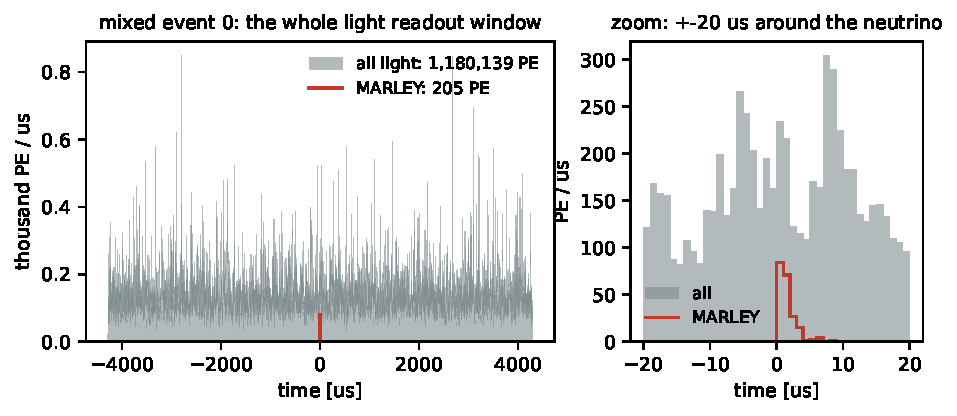
\includegraphics[width=\linewidth]{fig_overview_light.pdf}
\caption{Photoelectrons (PE) detected in one mixed event (stock simulation), per \textmu s. Grey: all light; red:
light from the MARLEY neutrino at $t=0$. Left: the whole $\pm$4.25\,ms light readout. Right: zoom on the neutrino.}
\label{fig:overview}
\end{figure}

\paragraph{What this means for the simulation.}
\begin{itemize}
\item \textbf{The background must be simulated in the same event as the signal} (``mixed'' events). Signal and
  background share photon detectors and electronics: pulses overlap, triggers merge, noise is shared. Simulating them
  separately and adding the outputs is not the same thing.
\item \textbf{The readout is long}: 8\,500 TPC samples of 0.5\us\ = 4.25\,ms for the charge, $\pm$4.255\,ms for the
  light. The light window is wider because the charge of a neutrino can arrive up to one drift time (4\,ms) after its
  light.
\item \textbf{The light matters more.} The flash gives the neutrino time, which is needed to know how far the charge
  drifted, i.e.\ its position and its energy (charge lost to impurities on the way). With $\sim$1\,000 flashes per
  readout, picking the right flash (charge--light matching) is the central problem of the low-energy reconstruction.
\item \textbf{Code paths that never see pile-up in beam samples see it constantly here.} Bugs B and C are of this
  kind: invisible in signal-only samples, large in mixed ones.
\end{itemize}

\begin{table}[H]\centering\small
\caption{Beam versus low-energy workflow.}
\begin{tabularx}{\linewidth}{@{}l X X@{}}
\toprule
 & beam & low energy (solar, supernova) \\
\midrule
signal energy & 0.5--10\,GeV & 5--30\,MeV \\
time of the interaction & known (beam spill) & unknown; self-trigger on light or charge \\
background per readout & negligible next to the signal & $\sim$130\,000 radioactive decays, \numAmixpe\ PE of
  light against \numAsolmarley\ PE from a solar $\nu$ \\
simulation unit & one interaction & signal + background in one readout (``mixed'') \\
generator & GENIE & MARLEY + DUNE radiological model (Decay0/RadioGen) \\
role of the light & $t_0$, trigger & $t_0$, energy, and picking 1 flash out of $\sim$1\,000 \\
reconstruction (official) & standard reco1/reco2 & \code{solar\_reco}: \code{gaushit}, \code{ophit10ppm},
  \code{SolarOpFlash}, \code{SolarCluster}, \code{SolarEvent}, analysis in \code{SolarNuAna} \\
\bottomrule
\end{tabularx}
\end{table}

The official low-energy reconstruction (S.~Manthey Corchado, DUNE solar group) lives in the packages
\fn{dunereco/LowEUtils}, \fn{duneopdet/LowEPDSUtils} and \fn{duneana/SolarNuAna}.
Its job files are
\fn{solar_reco_dunevd10kt_1x8x14_3view_30deg.fcl} (FD-VD) and \fn{solar_reco_dune10kt_1x2x6.fcl} (FD-HD).
This note stops at the OpHits, which are the input of that reconstruction.

%=====================================================================================================================
\section{The light simulation workflow}
\label{sec:workflow}
%=====================================================================================================================

\subsection{The detector}
The geometry is the FD-VD workspace \code{dunevd10kt\_1x8x14\_3view\_30deg}: one drift volume of the vertical-drift
module (2.56\,kt of argon, 6.5\,m drift), read out by 8$\times$14 = 112 charge-readout modules at the top and
\textbf{184 X-ARAPUCA photon detectors}: 112 on the cathode, 56 on the long side walls and 16 on the short ones. The
argon is doped with 10\,ppm of xenon, which shifts part of the slow argon light to xenon light. Every photon detector
(``OpDet'') is read by one electronics channel (``OpChannel'').

\subsection{The chain, step by step}

\begin{figure}[H]\centering
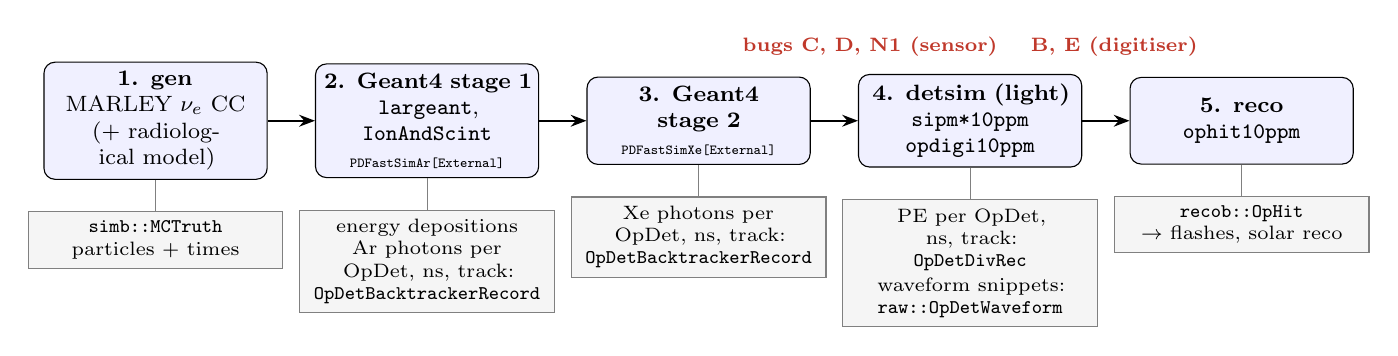
\begin{tikzpicture}[node distance=4mm and 6mm, font=\footnotesize,
  stp/.style={draw, rounded corners, fill=blue!6, align=center, minimum height=11mm, text width=26mm},
  prod/.style={draw=gray, fill=gray!8, align=center, text width=30mm, font=\scriptsize},
  arr/.style={-{Stealth[length=2mm]}, thick}]
\node[stp] (gen) {\textbf{1. gen}\\MARLEY $\nu_e$ CC\\(+ radiological model)};
\node[stp, right=of gen] (g4a) {\textbf{2. Geant4 stage 1}\\\code{largeant}, \code{IonAndScint}\\{\tiny\code{PDFastSimAr[External]}}};
\node[stp, right=of g4a] (g4b) {\textbf{3. Geant4 stage 2}\\{\tiny\code{PDFastSimXe[External]}}};
\node[stp, right=of g4b] (det) {\textbf{4. detsim (light)}\\\code{sipm*10ppm}\\\code{opdigi10ppm}};
\node[stp, right=of det] (rec) {\textbf{5. reco}\\\code{ophit10ppm}};
\foreach \a/\b in {gen/g4a, g4a/g4b, g4b/det, det/rec} \draw[arr] (\a) -- (\b);
\node[prod, below=of gen] (p1) {\code{simb::MCTruth}\\particles + times};
\node[prod, below=of g4a] (p2) {energy depositions\\Ar photons per OpDet, ns, track:\\\code{OpDetBacktrackerRecord}};
\node[prod, below=of g4b] (p3) {Xe photons per OpDet, ns, track:\\\code{OpDetBacktrackerRecord}};
\node[prod, below=of det] (p4) {PE per OpDet, ns, track:\\\code{OpDetDivRec}\\[1pt]waveform snippets:\\\code{raw::OpDetWaveform}};
\node[prod, below=of rec] (p5) {\code{recob::OpHit}\\$\to$ flashes, solar reco};
\foreach \a/\b in {gen/p1, g4a/p2, g4b/p3, det/p4, rec/p5} \draw[gray] (\a) -- (\b);
\node[font=\scriptsize\bfseries, text=bef, above=1mm of det] {bugs C, D, N1 (sensor) \quad B, E (digitiser)};
\end{tikzpicture}
\caption{The FD-VD light simulation chain (dunesw \code{v10\_26\_00d00}) and the product each step writes. The
bugs of this note live in step 4.}
\label{fig:chain}
\end{figure}

\begin{enumerate}[leftmargin=*]
\item \textbf{Generation.} MARLEY produces the electron and $\gamma$s of one solar $\nu_e$ CC interaction at $t=0$,
  at a random point in the active volume, with a flat 2--30\,MeV neutrino energy (physical spectra are obtained by
  reweighting). For mixed events, about 30 more generator modules add the radiological decays of the DUNE model,
  spread uniformly over $\pm$4.25\,ms. Job: \fn{prodmarley_solar_cc_flat[_radiological_decay0]_dunevd10kt_1x8x14_3view_30deg.fcl}.
\item \textbf{Geant4, stage 1.} Tracks every particle through the argon (\code{largeant}), converts the energy
  depositions into ionisation electrons and scintillation photons (\code{IonAndScint}), drifts the electrons
  (\code{elecDrift}) and computes how many \emph{argon} scintillation photons reach each OpDet and when
  (\code{PDFastSimAr}; \code{PDFastSimArExternal} for light made outside the field cage). Photons are not tracked one
  by one: a semi-analytic model (inside the field cage) or a photon library (outside) gives the fraction of photons
  from each point that reaches each OpDet. Only 5\,\% of the physical photons are simulated (\code{ScintPreScale}
  0.05); the sensor simulation corrects for it. The output, \code{OpDetBacktrackerRecord} (``BTR''), is a list per
  OpDet of (arrival time in ns, Geant4 track ID, number of photons). One such entry is an ``SDP''.
\item \textbf{Geant4, stage 2.} The same for the xenon light (\code{PDFastSimXe}, \code{PDFastSimXeExternal}).
\item \textbf{Light detector simulation} (``detsim''). Two kinds of modules:
  \begin{itemize}
  \item \code{SIPMOpSensorSim}, run four times (\code{sipmAr10ppm}, \code{sipmXe10ppm}, \code{sipmAr10ppmExt},
    \code{sipmXe10ppmExt}), one per BTR product. It decides which photons become photoelectrons (PE): detection
    efficiency 0.027 (3\,\% X-ARAPUCA $\times$ 90\,\% mesh transmission), a wavelength correction (0.65 for Ar
    light, 0.69 for Xe light), for Ar light a ``late light'' factor 0.31 (bug~C), SiPM cross-talk (20\,\% chance
    that one PE becomes two), and dark counts (10\,Hz, bug~D). Output: \code{OpDetDivRec}, the PE per OpDet, time
    and track.
  \item \code{WaveformDigitizerSim} (\code{opdigi10ppm}) turns the PE of all four products into one waveform per
    channel: 62.5\,MHz (16\,ns samples), a 10\,ADC pulse per PE that decays in 0.2\us, pedestal 500, line noise
    2.6\,ADC RMS, 14 bits. To save time, it only simulates the samples around PE pulses (``focus ranges'', bug~B).
    It then mimics the DAPHNE self-trigger: when the waveform rises by more than 1.5\,PE within 10 samples, it stores
    a 320-sample snippet starting 20 samples before the trigger (bug~E). Output: \code{raw::OpDetWaveform}, the
    snippets.
  \end{itemize}
\item \textbf{OpHit finding.} \code{ophit10ppm} (\code{OpHitFinder} with larana's \code{AlgoSiPM}) finds pulses above
  15\,ADC that stay above threshold for at least 60 samples, and converts their area into PE
  (area/130 + 0.43). Output: \code{recob::OpHit}. Flash finding and the solar reconstruction start from here.
\end{enumerate}

\subsection{Running it: the minimum workflow}
\label{sec:run}
All code is in \code{FD-LE/00-op-sim-debug/work} (\href{https://github.com/HaiwangYu/FD-LE}{\code{github.com/HaiwangYu/FD-LE}}). dunesw \code{v10} is built for
Scientific Linux 7; on the AlmaLinux 9 \code{dunegpvm}/\code{dunebuild} machines every LArSoft command runs inside
the Fermilab SL7 container, which \code{env/in-sl7.sh} starts and sets up. One event through the whole chain:
\begin{lstlisting}
cd FD-LE/00-op-sim-debug/work
scripts/run_chain.sh sol 0        # solar-only event 0:   ~2.5 min,  1 GB
scripts/run_chain.sh mix 0        # mixed event 0:        ~10 min,   6.2 GB peak (Geant4)
\end{lstlisting}
Each call runs the five steps above with the official job files (light-only versions of detsim and reco in
\code{fcl/}) and writes \code{data/events/<sol|mix>/evt<i>/reco.root}. Seeds are fixed per event and step
(\code{masterSeed} = 100000/200000 + 10\,$\times$\,index + step, Xin Qian's scheme), so event \code{mix 0} here is the
same event as in his samples: we reproduce his numbers for it to the last digit (section~\ref{sec:validation}).

To compare simulation versions on identical photons, the light simulation is \emph{rerun} from the BTRs kept in
\code{reco.root}, with the event's own detsim seed:
\begin{lstlisting}
scripts/build_duneopdet.sh        # duneopdet v10_26_00d00 + patches/duneopdet-light-sim-fixes.patch (~2 min)
scripts/run_rerun.sh stock mix 0  # CVMFS build
scripts/run_rerun.sh fixB  mix 0  # patched build, only the fix for bug B switched on
scripts/run_all.sh                # everything in this note: 20+20 events x 8 configurations + plots (~1.5 h)
\end{lstlisting}
To look inside an art file (from \code{env/in-sl7.sh bash}): \code{lar -c eventdump.fcl -s reco.root -n 1} lists the
data products, \code{config\_dumper -P reco.root} prints the configuration each job ran with, and the
\code{gallery} Python bindings used in \code{analysis/dump\_light.py} read products without writing an art job.

The configurations are listed in table~\ref{tab:configs}. Each rerun ends with \code{analysis/dump\_light.py}, which
writes the numbers per event (\code{light.npz}); \code{analysis/make\_plots.py} makes every figure and number of this
note (\code{numbers.tex}).

\begin{table}[H]\centering\small
\caption{Rerun configurations. ``legacy'' is the patched build with every switch at its old value; it differs from
the stock build only by the fix for bug~E, which has no switch. Each \code{fix*} configuration switches on one fix.}
\label{tab:configs}
\begin{tabular}{@{}l l l@{}}
\toprule
configuration & build & settings \\
\midrule
\code{stock}   & CVMFS \code{duneopdet v10\_26\_00d00} & -- \\
\code{legacy}  & patched & all switches legacy (E fixed) \\
\code{fixB}    & patched & legacy + \code{MergeOverlappingRanges: true} \\
\code{fixC}    & patched & legacy + \code{LateLightReference: "Track"} (Ar products) \\
\code{fixD}    & patched & legacy + \code{DarkNoiseTimeInNs: true} \\
\code{fixN1}   & patched & legacy + \code{BinomialQE: true} \\
\code{default} & patched & the proposed defaults: B, D, E, N1 fixed, C legacy \\
\code{all}     & patched & default + \code{LateLightReference: "Track"} \\
\bottomrule
\end{tabular}
\end{table}

%=====================================================================================================================
\section{The bugs, their impact, and the fixes}
\label{sec:bugs}
%=====================================================================================================================

The samples: solar-only events 0--19 and mixed events 0--19 (\numNsol\ + \numNmix). Per event the stock simulation
gives \numAsolmarley\ PE (solar-only, all MARLEY) and \numAmixpe\ PE (mixed), \numAmixsnip\ snippets and
\numAmixhits\ OpHits. ``Before'' is the \code{legacy} configuration and ``after'' the matching \code{fix*}
configuration, except for bug~E (stock versus legacy).

%---------------------------------------------------------------------------------------------------------------------
\subsection{Bug B --- overlapping focus ranges: samples stored twice, duplicate OpHits, double noise}
%---------------------------------------------------------------------------------------------------------------------

\bugbox{
For each PE, \code{WaveformDigitizerSim} marks a ``focus range'' (the pulse plus 100 samples of margin on each side)
in which it adds noise and looks for triggers. \code{FocusList::AddRange} is meant to merge ranges that overlap, but it
misses two cases: a new range that \emph{contains} an old one is added as a second range, and a range that grows until
it reaches its neighbour is never merged with it. Everything after that loops over the ranges, so in an overlap the
noise is added twice and the trigger fires twice on the same samples: the same piece of waveform is stored in two
snippets, and the OpHit finder finds the same pulse twice.}{
Overlaps need many PE close in time on one channel, which only the radiological background provides: solar-only
events are unaffected, in mixed events \numBlegacymixagain\,\% of the stored samples are copies,
\numBlegacymixduphits\,\% of the OpHits are duplicates and they carry \numBlegacymixduppe\,\% of the OpHit PE. The
duplication does not care where the light came from: \textbf{signal pulses are duplicated too}. The doubled noise
(median baseline RMS \numBlegacymixrms\ instead of \numBfixBmixrms\,ADC) fires extra triggers: removing the duplicate
hits after the fact leaves \numBlegacymixdedhits\ hits and \numBlegacymixdedupe\ PE, still more than the
\numBfixBmixhits\ hits and \numBfixBmixhitpe\ PE of the fixed simulation.}{
A new \code{FocusList.h}: \code{AddRange} merges the new range with every range it overlaps (one pass; the ranges are
disjoint before each call). If no range ever overlapped, the result, including the order of the ranges, is exactly the
legacy one, so events without overlaps are bit-identical. Switch \code{MergeOverlappingRanges} (default \code{true};
\code{false} = legacy). A unit test (\code{FocusList\_test}, 2\,000 random pile-up trials) checks both properties.}

\begin{figure}[H]\centering
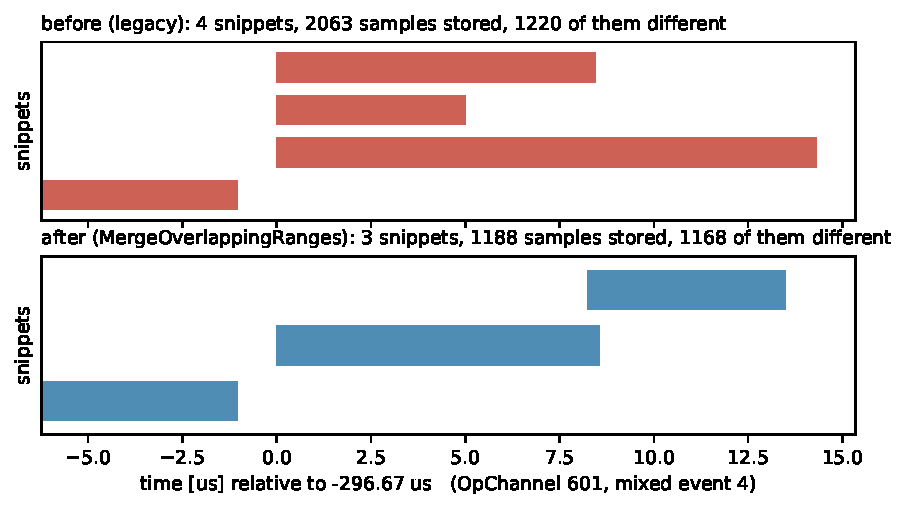
\includegraphics[width=0.86\linewidth]{fig_B_snippets.pdf}
\caption{Bug B on one channel of a mixed event: the stored snippets (one bar each) before and after the fix. Before,
three snippets start on the same tick and store the same samples again. After, every sample is stored once, except the
20-sample pre-trigger of a snippet that opens right after the previous one closed (N6 in section~\ref{sec:other}).
This place was chosen because both versions read out the same samples there; elsewhere the readouts also differ
because the doubled noise of the legacy version fires extra triggers.}
\end{figure}
\begin{figure}[H]\centering
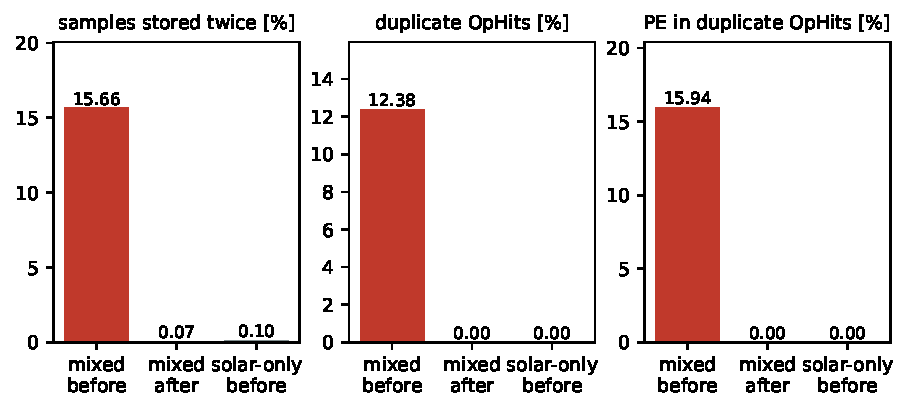
\includegraphics[width=\linewidth]{fig_B_summary.pdf}\\[2mm]
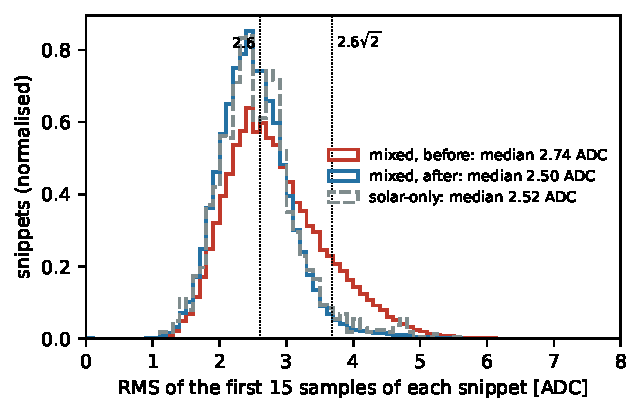
\includegraphics[width=0.6\linewidth]{fig_B_noise.pdf}
\caption{Bug B, all events. Top: fraction of samples stored twice, of duplicate OpHits (same channel and peak time)
and of the OpHit PE they carry, before and after the fix. The \numBfixBmixagain\,\% of samples still stored twice after the fix are the 20-sample
pre-trigger of a new snippet re-reading the end of the previous one, which is how the readout is modelled.
Bottom: baseline noise of the snippets; the noise is added twice where ranges overlap (expected RMS
$2.6\sqrt2 = 3.7$\,ADC).}
\end{figure}

%---------------------------------------------------------------------------------------------------------------------
\subsection{Bug C --- the ``late light'' clock starts at the first photon of the whole event}
%---------------------------------------------------------------------------------------------------------------------

\bugbox{
In xenon-doped argon most of the slow argon light is converted into xenon light, so only a part of it arrives as argon
light. \code{SIPMOpSensorSim} models this with the arrival time: argon photons that arrive within 10\,ns of a reference
time keep their weight, later ones are scaled by 0.31. The model only makes sense if the reference is the start of the
\emph{same} interaction's light, but the code takes the first photon on that OpDet in the \emph{whole event}
($\pm$4.25\,ms). In a mixed event that is a background photon, usually milliseconds before the neutrino, so all argon
light of the neutrino, its prompt light included, is treated as late. (A loop meant to find the first time does
nothing; it is harmless because the list is already time-ordered.)}{
Solar-only events are unaffected (the first photon is the neutrino's own). In mixed events MARLEY gets
\numClegacymixratio\ argon PE per argon photon instead of \numClegacysolratio. The per-track reference (the fix) raises
the MARLEY light (argon and xenon) by \numCgainsolmarley\,\% in solar-only and by \numCgainmixmarley\,\% in mixed
events, and the total light of mixed events by \numCgainmixtotal\,\%: the background is dimmed the same way.}{
Switch \code{LateLightReference}: \code{"Event"} (default, legacy) or \code{"Track"}: the reference is the first photon
of the same Geant4 track on that OpDet. Tracks of one interaction start within ns of each other; a delayed process
(neutron capture, decay) gets its own reference. Per track is slightly more generous than per interaction (each track
of a MARLEY event gets its own 10\,ns window); an exact per-interaction reference would need the MC-truth grouping,
which the module does not have. We propose \code{"Track"} but leave the choice to the light-simulation experts, as it
changes the light yield of every sample with xenon doping.}

\begin{figure}[H]\centering
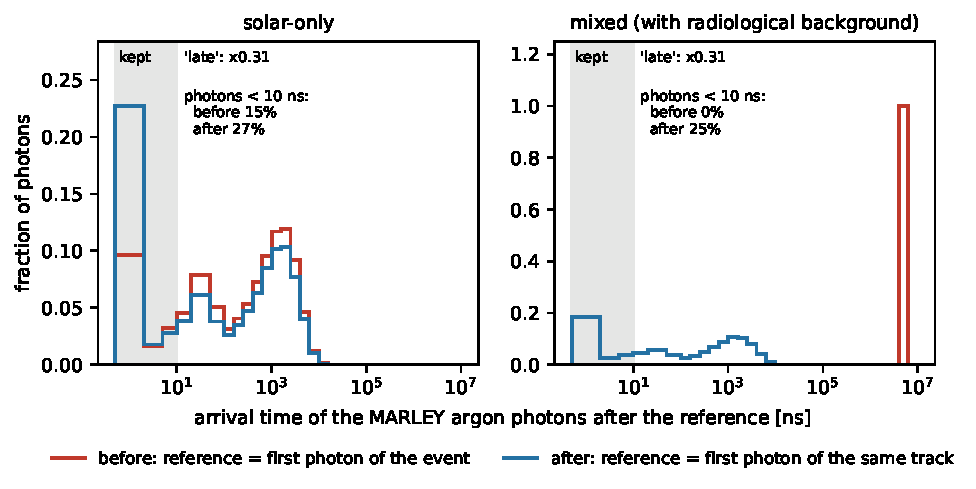
\includegraphics[width=\linewidth]{fig_C_arrival.pdf}
\caption{Bug C: arrival time of the MARLEY argon photons after the reference time, with the event's first photon on
the OpDet as reference (legacy, red) and with the first photon of the same track (fix, blue). Photons in the grey
band keep their weight, later ones get $\times0.31$. In mixed events (right) no MARLEY photon is within 10\,ns of the
event reference.}
\end{figure}
\begin{figure}[H]\centering
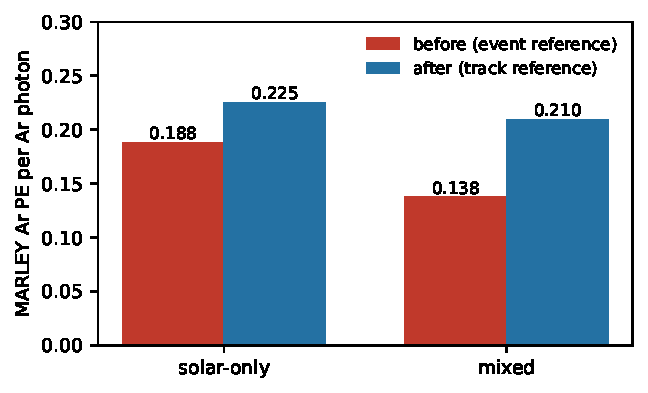
\includegraphics[width=0.55\linewidth]{fig_C_yield.pdf}
\caption{Bug C: MARLEY argon PE per simulated argon photon, before and after the fix. Before, the same neutrino gives
\numCgainmixratio\ of its per-track argon light in mixed events; after, the two samples agree within the statistics of
\numNmix\ events.}
\end{figure}

%---------------------------------------------------------------------------------------------------------------------
\subsection{Bug D --- dark counts all land on the neutrino}
%---------------------------------------------------------------------------------------------------------------------

\bugbox{
\code{SIPMOpSensorSim::AddDarkNoise} draws dark-count times over the readout window, with the window and the mean
spacing in \textmu s, and stores them in the \code{OpDetDivRec}, whose times are in ns. The right number of dark
counts is drawn, but squeezed 1000$\times$ in time: all of them fall within $\pm$4.25\us\ of $t=0$, which is where
the neutrino is.}{
\numDperevent\ dark PE per event (\numDlegacyn\ in the \numNsol+\numNmix\ events, from \numDlegacymin\ to
\numDlegacymax\us) are piled on the signal flash instead of being spread over the $-4.04$ to $+4.25$\,ms range the
code intends. They are single
PE on many channels, so few make OpHits (Xin Qian measured $\sim$1\,\% on the MARLEY OpHit PE, doc 14), but they bias
any study of the flash at the neutrino time, and the effect grows with the dark rate.}{
Switch \code{DarkNoiseTimeInNs} (default \code{true}): the time is converted to ns before it is stored.}

\begin{figure}[H]\centering
\includegraphics[width=\linewidth]{fig_D_dark.pdf}
\caption{Bug D: times of the dark-count PE, all events, before and after the fix (grey: the light readout window).}
\end{figure}

%---------------------------------------------------------------------------------------------------------------------
\subsection{Bug E --- readout start underflows at the beginning of the window}
%---------------------------------------------------------------------------------------------------------------------

\bugbox{
The self-trigger opens a snippet 20 samples before the trigger sample: \code{wstart = tick - PreTrigger}. Both are
unsigned integers, so a trigger in the first 20 samples of the window gives $2^{64}-k$ instead of a negative number.
The snippet gets the time stamp \numEwrapvalue\us, and it is copied from memory before the start of the waveform
buffer (an out-of-bounds read, and possibly a write, since the digitiser clamps saturated samples in place).}{
Only mixed events have light at the very start of the window: \numEstockmixsnip\ such snippets in the \numNmix\ mixed
events (\numEstockmixhits\ OpHits at that time), none in solar-only events. Small in physics terms, the hits are easy to
drop, but it is undefined behaviour.}{
Clamp the start at the first sample. No switch: the legacy output cannot be reproduced reliably anyway. After the fix
the same triggers give normal snippets that start at the first sample of the window ($-4255$\us).}

\begin{figure}[H]\centering
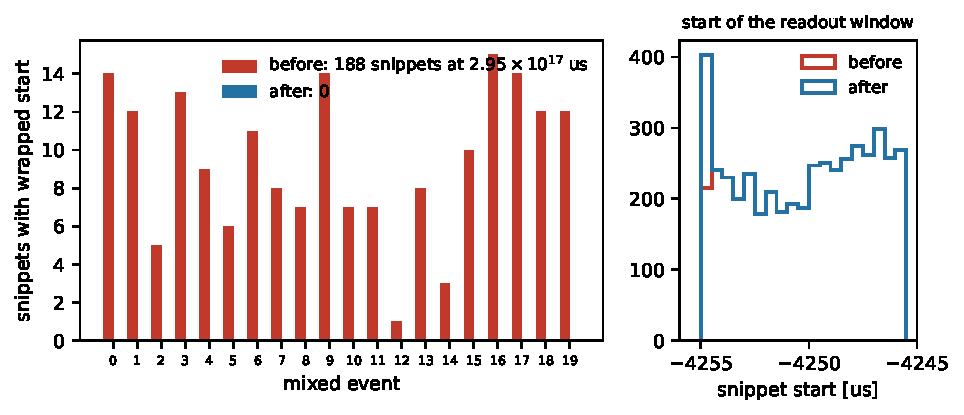
\includegraphics[width=\linewidth]{fig_E_wrapped.pdf}
\caption{Bug E. Left: snippets with a wrapped start time per mixed event, before and after the fix. Right: snippet
start times at the beginning of the window; after the fix the same triggers give snippets that start at $-4255$\us.}
\end{figure}

%---------------------------------------------------------------------------------------------------------------------
\subsection{Bug N1 --- photon detection is Poisson on top of Poisson}
%---------------------------------------------------------------------------------------------------------------------

\bugbox{
\code{PDFastSim} already draws the number $N$ of photons that reach an OpDet as a Poisson number. \code{SIPMOpSensorSim}
then draws the detected photons as $\mathrm{Poisson}(qN)$ (with $q = \numNq$ for xenon light) instead of detecting
each of the $N$ photons with probability $q$ (binomial). The mean is right, the spread is not: one photon can give two
detected photons, and $P(0\,|\,N=1) = e^{-q} = \numNpredpoisson$ instead of $1-q = \numNpredbinomial$.}{
The PE per OpDet fluctuate more than physically possible (variance $\times(1+q)/(1-q)$ before cross-talk). Every
mean-based calibration agrees with the legacy simulation, so it hid; it matters for resolutions and for any study of
small signals.}{
Switch \code{BinomialQE} (default \code{true}): \code{CLHEP::RandBinomial(N, q)}. Different random numbers, so not
bit-identical to the legacy output when on.}

\begin{figure}[H]\centering
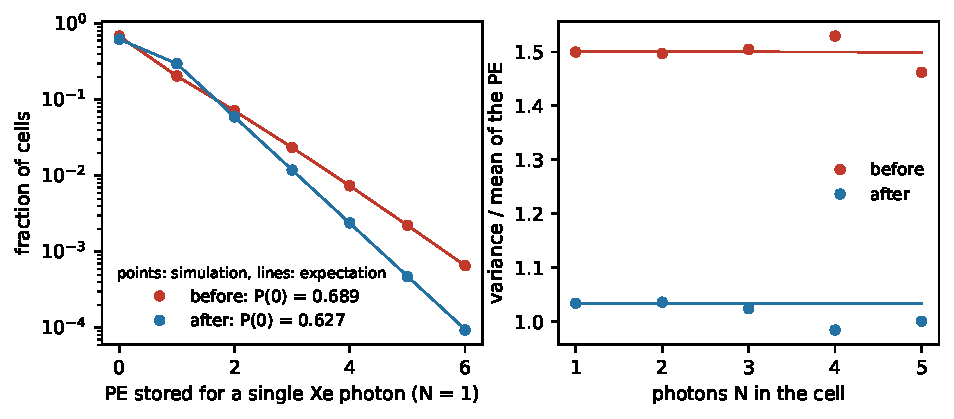
\includegraphics[width=\linewidth]{fig_N1_qe.pdf}
\caption{Bug N1, measured on the xenon-light cells that hold exactly one Geant4 entry with $N$ photons
(\numNlegacycells\ cells with $N=1$). Left: PE stored for a single photon; lines: the expectation of each model with
20\,\% cross-talk. Right: variance over mean of the stored PE versus $N$.}
\end{figure}

%---------------------------------------------------------------------------------------------------------------------
\subsection{All fixes together}
%---------------------------------------------------------------------------------------------------------------------

\begin{table}[H]\centering\small
\caption{Totals over the samples with the stock build, the proposed defaults, and all fixes including the per-track
late light. OpHits with a wrapped time (bug E) are not counted.}
\label{tab:all}
\begin{tabular}{@{}l r r r r r r@{}}
\toprule
 & \multicolumn{3}{c}{solar-only (\numNsol)} & \multicolumn{3}{c}{mixed (\numNmix)} \\
\cmidrule(lr){2-4}\cmidrule(lr){5-7}
 & stock & default & all & stock & default & all \\
\midrule
PE (sensor output) & \numOstocksolpe & \numOdefaultsolpe & \numOallsolpe & \numOstockmixpe & \numOdefaultmixpe & \numOallmixpe \\
MARLEY PE & \numOstocksolmarley & \numOdefaultsolmarley & \numOallsolmarley & \numOstockmixmarley & \numOdefaultmixmarley & \numOallmixmarley \\
OpHits & \numOstocksolhits & \numOdefaultsolhits & \numOallsolhits & \numOstockmixhits & \numOdefaultmixhits & \numOallmixhits \\
OpHit PE & \numOstocksolhitpe & \numOdefaultsolhitpe & \numOallsolhitpe & \numOstockmixhitpe & \numOdefaultmixhitpe & \numOallmixhitpe \\
\bottomrule
\end{tabular}
\end{table}

In mixed events the proposed defaults leave the photoelectrons of the sensor simulation unchanged in total (N1 changes
only their fluctuations, D only the time of the dark counts) but remove \numBlegacymixduphits\,\% of the OpHits and
reduce the OpHit PE from \numOstockmixhitpe\ to \numOdefaultmixhitpe: the duplicates of bug B and the extra triggers
of its doubled noise. The per-track late light then adds \numCgainmixtotal\,\% of light. Solar-only events barely
change with the defaults; the per-track late light raises their MARLEY light by \numCgainsolmarley\,\%.

%=====================================================================================================================
\section{Other known issues of the chain (not fixed here)}
\label{sec:other}
%=====================================================================================================================

From Xin Qian's fdvd\_sim docs 03, 08 and 30; letters and numbers as there.
\begin{itemize}
\item \textbf{A} --- \code{OpFlashFinderVerticalDrift} (official \code{opflash10ppm}) mixes up time-sorted ranks and
  hit indices when it collects neighbours, so flashes are built from the wrong hits. Reconstruction, not simulation.
\item \textbf{F} --- \code{ophit10ppm} requires 60 samples (0.96\us) above threshold for a pulse that decays in
  0.2\us: most single-PE pulses never make a hit. A setting, and the largest light loss of the chain (Xin Qian: the
  hits keep 23\,\% of the PE).
\item \textbf{N2} --- dark noise is added once per sensor module (4 times, 40\,Hz in total) and only on OpDets that
  saw light.
\item \textbf{N3} --- \code{OpDetDivRec::AddPhoton} (dunecore) credits every photon at an existing time to the first
  track there; totals are right, per-track attribution is not (negligible in practice).
\item \textbf{N4} --- the residual argon light keeps the 1.6\us\ decay time of undoped argon.
\item \textbf{N5} --- \code{ophit10ppm} adds 0.43\,PE to every OpHit (\code{SPEShift}, tuned for FD-HD).
\item \textbf{N6} --- consecutive snippets of one range can overlap by up to 20 samples (the residual of bug B after
  the fix).
\item The same \code{FocusList::AddRange} as bug B is copied into five other digitisers, including the ProtoDUNE-HD and
  ProtoDUNE-VD ones; they would need the same fix and a ProtoDUNE validation.
\end{itemize}

%=====================================================================================================================
\section{Validation}
\label{sec:validation}
%=====================================================================================================================

\begin{itemize}
\item \textbf{The events are Xin Qian's events.} With his seeds, our mixed events 0 and 500 have 15\,028\,912 and
  14\,910\,646 samples stored twice and 31\,755 and 31\,970 snippets starting on the same tick as another, the numbers
  of his doc~08a.
\item \textbf{The rerun reproduces the stored simulation:} stock rerun versus the products of the original job
  (waveforms and the four \code{OpDetDivRec} products, compared by hash): \numgatestockeqstored.
\item \textbf{Each fix changes only what it should.}
  The legacy configuration differs from the stock build only in the snippets of bug~E (wrapped start before, start
  at the first sample after): \numgateEonly; its sensor output is identical: \numgatelegacydiveq.
  Fix B leaves the sensor output unchanged: \numgateBdiv; fix C leaves the xenon products unchanged: \numgateCxe.
  With fix B on, \numgateBidentsol\ solar-only events are bit-identical to the legacy output, including all
  \numgateBnolapsol\ that have no sample stored twice; the other solar-only events and all mixed events had
  overlapping ranges.
\item \textbf{Build:} the patch compiles with \code{-Werror} against dunesw \code{v10\_26\_00d00}, the unit test
  passes, and the patch applies unchanged to \code{duneopdet} \code{develop} (the two modules have not changed since
  \code{v10\_26\_00d00}).
\end{itemize}

\appendix
%=====================================================================================================================
\section{The patch}
\label{app:patch}
%=====================================================================================================================
The fixes are commit \code{6c73f2f} on branch \code{fix-light-sim-pileup} of the fork
\href{https://github.com/HaiwangYu/duneopdet/tree/fix-light-sim-pileup}{\code{github.com/HaiwangYu/duneopdet}},
on top of \code{DUNE/duneopdet} \code{develop} (\code{497d0a1}, 2026-10-06), ready for a pull request.
The same change is the patch \fn{work/patches/duneopdet-light-sim-fixes.patch}, which also applies to
\code{v10\_26\_00d00} and is what \fn{scripts/build_duneopdet.sh} builds:
\begin{itemize}
\item \code{OpticalDetector/FocusList.h} (new): \code{FocusList} moved out of \code{WaveformDigitizerSim\_module.cc},
  with the merging \code{AddRange} (B).
\item \code{WaveformDigitizerSim\_module.cc}: switch \code{MergeOverlappingRanges} (B); clamp of the snippet start (E).
\item \code{SIPMOpSensorSim\_module.cc}: switches \code{LateLightReference} (C), \code{DarkNoiseTimeInNs} (D),
  \code{BinomialQE} (N1); the dead loop removed.
\item \code{WaveformDigitizerSim.fcl}, \code{SIPMOpSensorSim.fcl}: the new switches with their defaults and comments.
\item \code{OpticalDetector/test/FocusList\_test.cc} (new): Boost unit test of the range merging.
\end{itemize}
To reproduce an existing sample bit for bit, set \code{MergeOverlappingRanges: false}, \code{DarkNoiseTimeInNs: false}
and \code{BinomialQE: false} (the output then differs only in the bug-E snippets).

%=====================================================================================================================
\section{Glossary}
%=====================================================================================================================
\begin{tabularx}{\linewidth}{@{}l X@{}}
art, fcl & the event-processing framework of LArSoft, and its configuration language \\
BTR, SDP & \code{OpDetBacktrackerRecord}: per OpDet, the photons from Geant4 by time and track; one entry is an SDP \\
DivRec & \code{OpDetDivRec}: per OpDet, the photoelectrons by time and track, after the sensor simulation \\
OpDet, OpChannel & a photon detector (here an X-ARAPUCA), and its electronics channel \\
PE & photoelectron: one detected photon (a SiPM signal of one unit) \\
snippet & a stored piece of waveform (\code{raw::OpDetWaveform}), 320 samples of 16\,ns by default \\
OpHit, flash & a pulse found in a snippet; a group of OpHits close in time on several OpDets \\
MARLEY & the generator of MeV neutrino--argon interactions \\
mixed event & a MARLEY event and the radiological background simulated together in one readout \\
mrb, ups & the tools that build (\code{mrb}) and set up (\code{ups}) LArSoft packages \\
\end{tabularx}

\paragraph{Acknowledgements.} The bugs were found by Xin Qian, who also wrote the light-only job files and the event
seeding used here. S.~Manthey Corchado described the official low-energy workflow. This note and its scripts were
drafted with an AI assistant (Claude) and checked against the simulation outputs.

\end{document}
